%% This is an example first chapter.  You should put chapter/appendix that you
%% write into a separate file, and add a line \include{yourfilename} to
%% main.tex, where `yourfilename.tex' is the name of the chapter/appendix file.
%% You can process specific files by typing their names in at the 
%% \files=
%% prompt when you run the file main.tex through LaTeX.
\chapter{WebAuthn Transaction Authentication}\label{Chap:WebauthnTransactionAuthentication}

%% Detailed diagram https://swimlanes.io/#nVPJTsNADL3nK/wBlA+oEFJbVXAACdECx8qZuMkozUyYcbr8Pc6mLKVAuUWTt9h+9qzghAxrhWwd3E0m9/BB4WTu7MGTm8LSM4Y77RNYWGNIsbYmCDZTWBEXOawYYwoCY5mGvIUjlDfs5IUIGXlfEXpYEMt3cnrbgpYmauVf6bMgzzcwG+o8tzqV8Tm7dTcROMooC8VGJbjboYkJgmDMgHHbixJMAr6B5ZHJeAF6OGhOqlLMbVfCprQ75Wxjh3miFcyYpWasJzVqdNYf91U2Vacj+lupqqzZapd5sDm5xnWAO2tupWODXDhxva7Pwdia6H9N8nG9fumC/J/3hZirlxNwglzHW6pBhqwS8uCld4q6HxdlHsiUk+tvq+ZuWyFELzryUI06LtopX1q+hFRaF+VIkd4LGeuGWsW2xLhxHgMuaj9Zm4IcRlGOOy/kMhWkdAJtIEK5VKn0qrp8GwdoD3vc6ej745ijSkk+V+T25Qr1Q20Mx5DlkVQhlzDCDmE/rozPZSHoD9c6wH8B

WebAuthn transaction authentication is a protocol specification for authenticating high-risk user operations after login. The specification describes a sequence of steps that must be followed in order to authenticate properly. There is registration and then transaction authentication, which can be split into three stages: the setup, the cryptographic attestation and then the verification. Figure~\ref{Fig:TxAuthnFlowOverview} gives a simplified overview of the transaction authentication process. It visualizes the order of communication among the hardware authenticator, the web-browser, the WebAuthn verification end and backend server.

%% 
%% \iffalse
%% These steps can be split into four stages: registration, the setup, the cryptographic attestation and then the verification.
%% Transaction authentication pertains to the setup, cryptographic attestation and verification stages. 
%% \fi
%% 

%% https://swimlanes.io/#jVJBbsIwELz7FfsA6ANQVSkgpF4qVQ1tj2hxltgiWaf2BsTva4cikpRSbpZndnZm7KwVQyxWozgPj9PpE3zSZjr37hDIz2AZBDeVDQYWjpm0WMdKrWeQk7QN5IIlKdUbgajwQd5uk2Qkw5KLM/uNvloKohQ7oSushSeMAHIBnmqqN1FOG6wq5JJAqfEEjN0uEpk4WVonuWMjrvTYGKshE4m78RRgZDjrt9CTmXQIP8ALhdAl7ZyP6O9JRTveWl8HcA35ny0D3i+zuS0ZpfUEBytm5H0Q9d6Wn1er13PJkxv6f9Tf3RxBDMqp9sSGGkUbChBiBiouwH8yl/V7rGxh5Xj9AeeodxSPOfl9qqUfQqkhejN2aBwHuuOXDPjf
%% Zoom out to 90% on web-browser and screenshot, convert to pdf
%% :screenshot --selector .diagram --filename /tmp/txauthn_flow.png (in firefox console)
\begin{figure}
  \centering
  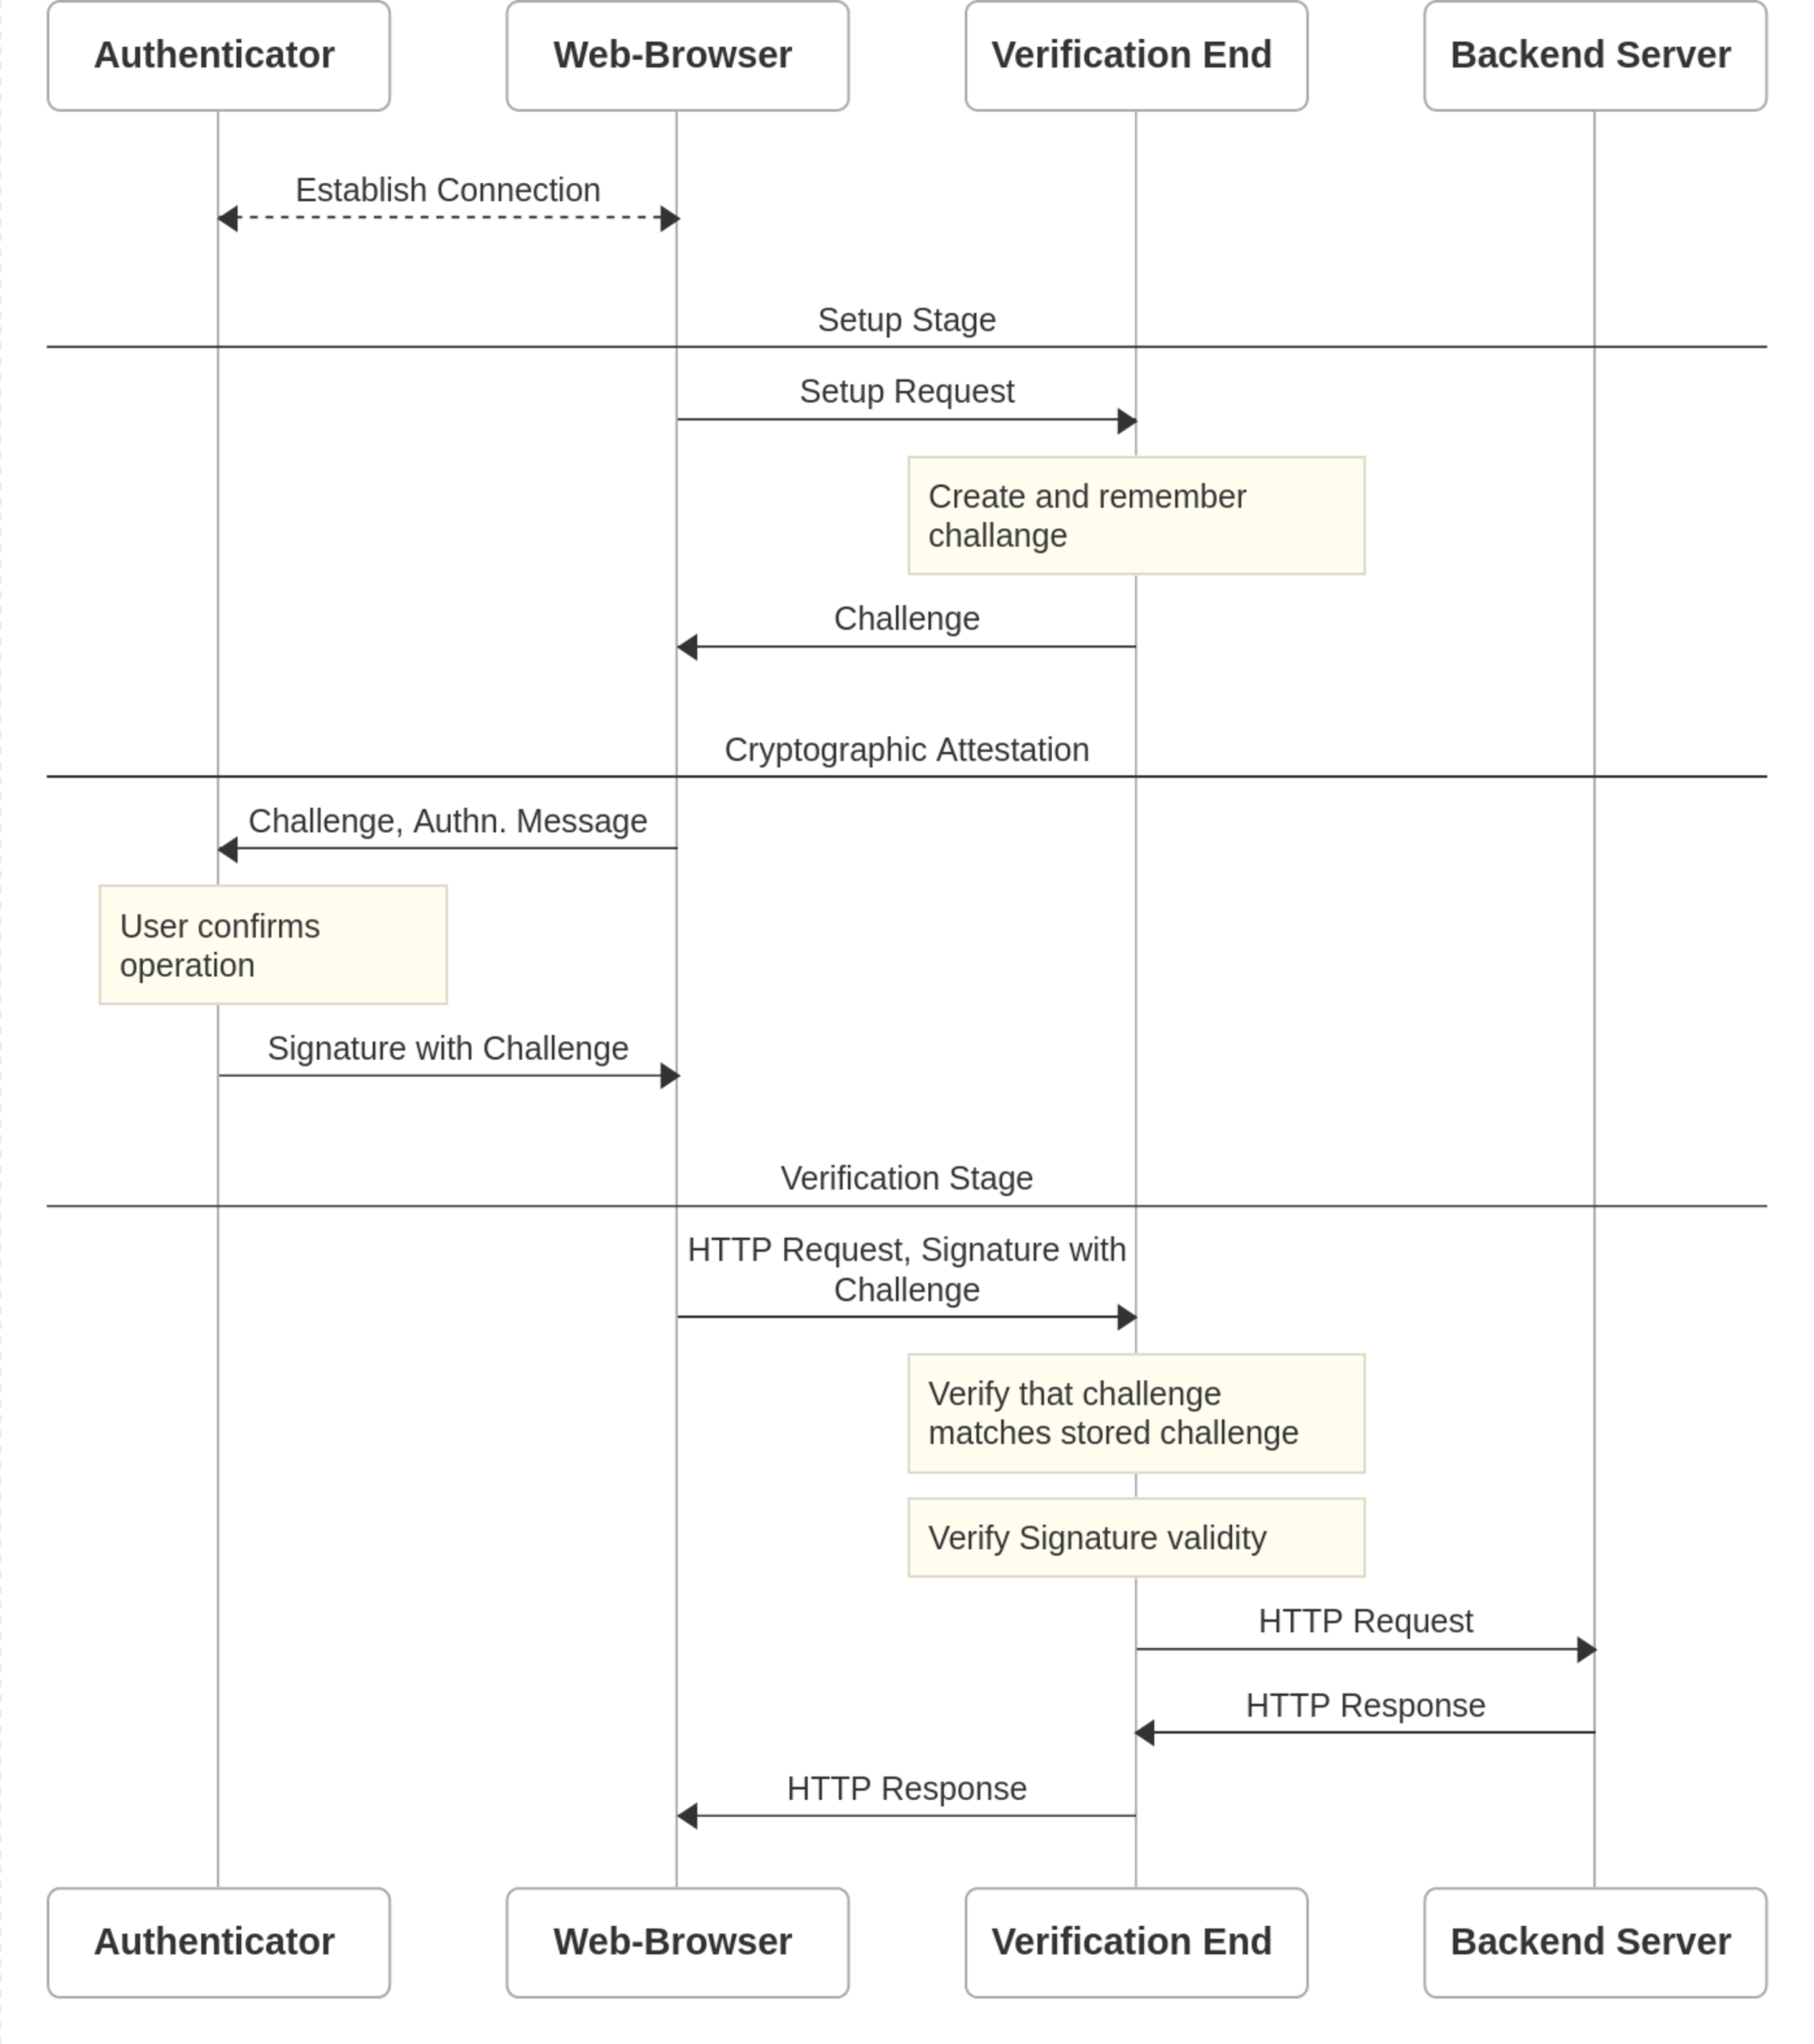
\includegraphics[width=16cm]{txauthn_flow_overview_swimlanes}
  \caption{A simplified overview of the flow of events during WebAuthn transaction authentication, subdivided into three stages.}
  \label{Fig:TxAuthnFlowOverview}
\end{figure}

%% 
%% \iffalse
%% store later accessible to the verification code and is performed only once per user.
%% \fi
%% 

\begin{enumerate}[nosep]
\item Registration: Makes a record of the user and their cryptographic credential into a database. Registration is performed only once per user and is assumed secure. The database record is used by the verification step later on.

\item Setup: Initiated by the user's web-browser and involves a priming exchange between it and the WebAuthn verification end.

\item Cryptographic Attestation: Occurs on the hardware authenticator device after the user confirms the operation. The threat model assumes that this attestation is secure.

\item Verification: Validates whether to authorize the high-risk user operation or not. Checks if the requested operation matches its authentication message and that the cryptographic signature on it is valid. This stage also is assumed secure under the threat model.

\end{enumerate}

The rest of this chapter describes these steps in more detail and uses \sys{}, the WebAuthn firewall, as the verification end. It contains the database of user public key credentials and performs the validation to authorize high-risk operations or not. 

%% 
%% \iffalse
%% This outline for transaction authentication 

%% As webauthn is a protocol specification, nothing dictates this design choice. However, for continuity with the thesis work, the protocol is best explained with the firewall.
%% \fi
%% 

%% 
%% \iffalse
%% between the user and hardware authenticator device. 

%% Lastly, the verification stage 
%% Occurs within the firewall, and it 
%% \fi
%% 

\section{WebAuthn Registration}

%% https://swimlanes.io/#fZFNboMwEIX3PsUcoFwgqioliFU3FZWa9WC/BEtgt/aQiNtnSDYQSrZ+P36fZj9IiyDessRE70XxQUc0xSHFa0baUZWFm87nlsoYAqz4GIyZWUgTP0j+NFWoSFVwO/qGDL9U429AFmNCFPzjKhNYBQ6OEnr0jdbZlruOwxlkzHOCnteVkxlqXk3az7kWxoWyavwalNbSJ8a3F+1rlI3cBvj9ZVRoC3+Be0BPCepZbItMWcfNhc2qGjYmN/ufJJJjvRpn3AA=
%% Zoom in to 200% on web-browser and screenshot, convert to pdf
\begin{figure}[h]
  \centering
  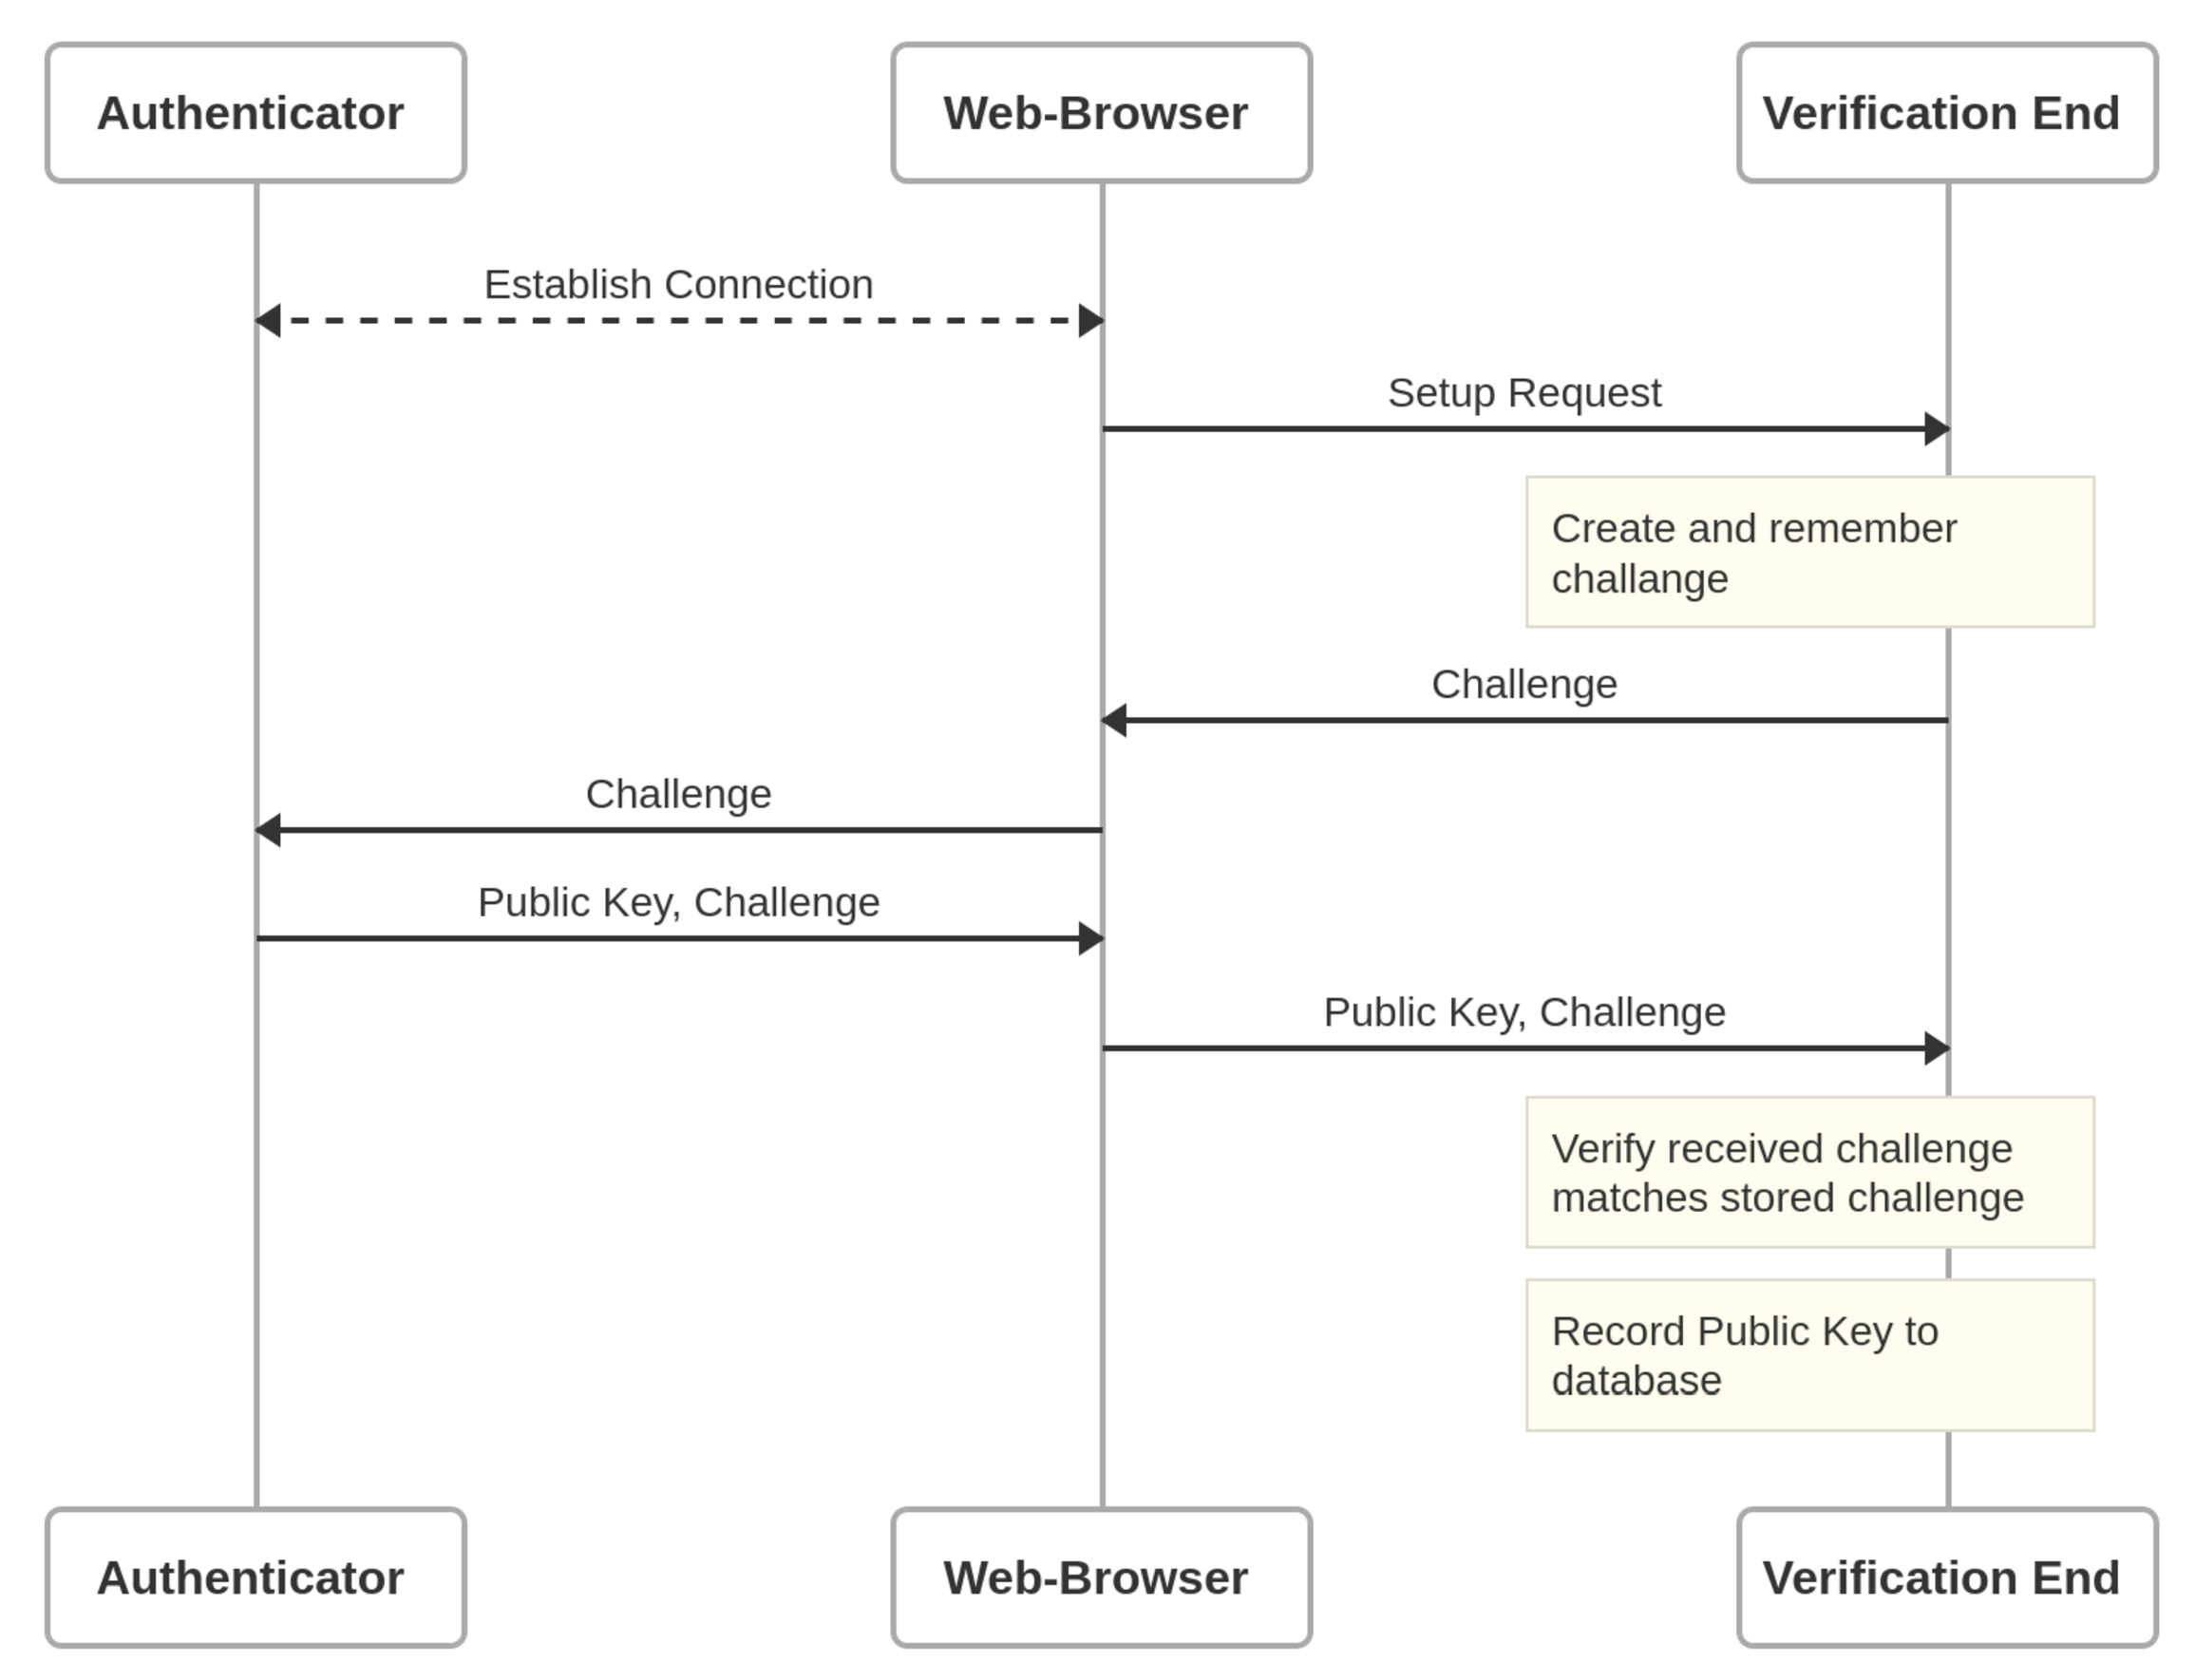
\includegraphics[width=16cm]{registration_flow_swimlanes}
  \caption{The flow of events during WebAuthn registration.}
  \label{Fig:WebauthnRegistrationFlow}
\end{figure}

The purpose of registration is for the user's hardware device to transfer its public key credential to \sys{}. This process is assumed to be secure in the threat model, with no adversary able to intercept or tamper with any of the communications. Therefore, whatever credential \sys{} receives during registration is assumed to be genuine and the user's. The firewall later on uses this credential during the verification stage to ensure transaction authentication integrity. 

%% 
%% \iffalse
%% \begin{lstlisting}
%% type PublicKeyCredentialCreationOptions struct {
%% 	Challenge              Challenge                
%% 	RelyingParty           RelyingPartyEntity       
%% 	User                   UserEntity               
%% 	Parameters             []CredentialParameter
%% 	AuthenticatorSelection AuthenticatorSelection
%% 	Timeout                int                      
%% 	Attestation            ConveyancePreference
%% }
%% \end{lstlisting}
%% \fi
%% 

Figure~\ref{Fig:WebauthnRegistrationFlow} illustrates the flow of events during the registration event. The registration process begins with a setup of its own, where the web-browser requests a few parameters from the firewall, most notably a random challenge nonce. \sys{} remembers the challenge it sent as a part of the session data associated with the registration setup request. The challenge nonce prevents replay attacks. There are a few other parameters, but they are mainly for the hardware device to know what type of credential the firewall is expecting to receive. The hardware device sends over its public key credential for \sys{} to save, with the challenge signed by that credential. \sys{} receives an HTTP POST request containing this public key credential. The POST request also contains identifying information of the current user. \sys{} verifies that the challenge is matches, and upon success, stores the credential and associated user ID into a database row.

\section{Transaction Authentication Setup}\label{Sec:TransactionAuthenticationSetup}

\begin{figure}
  \centering
  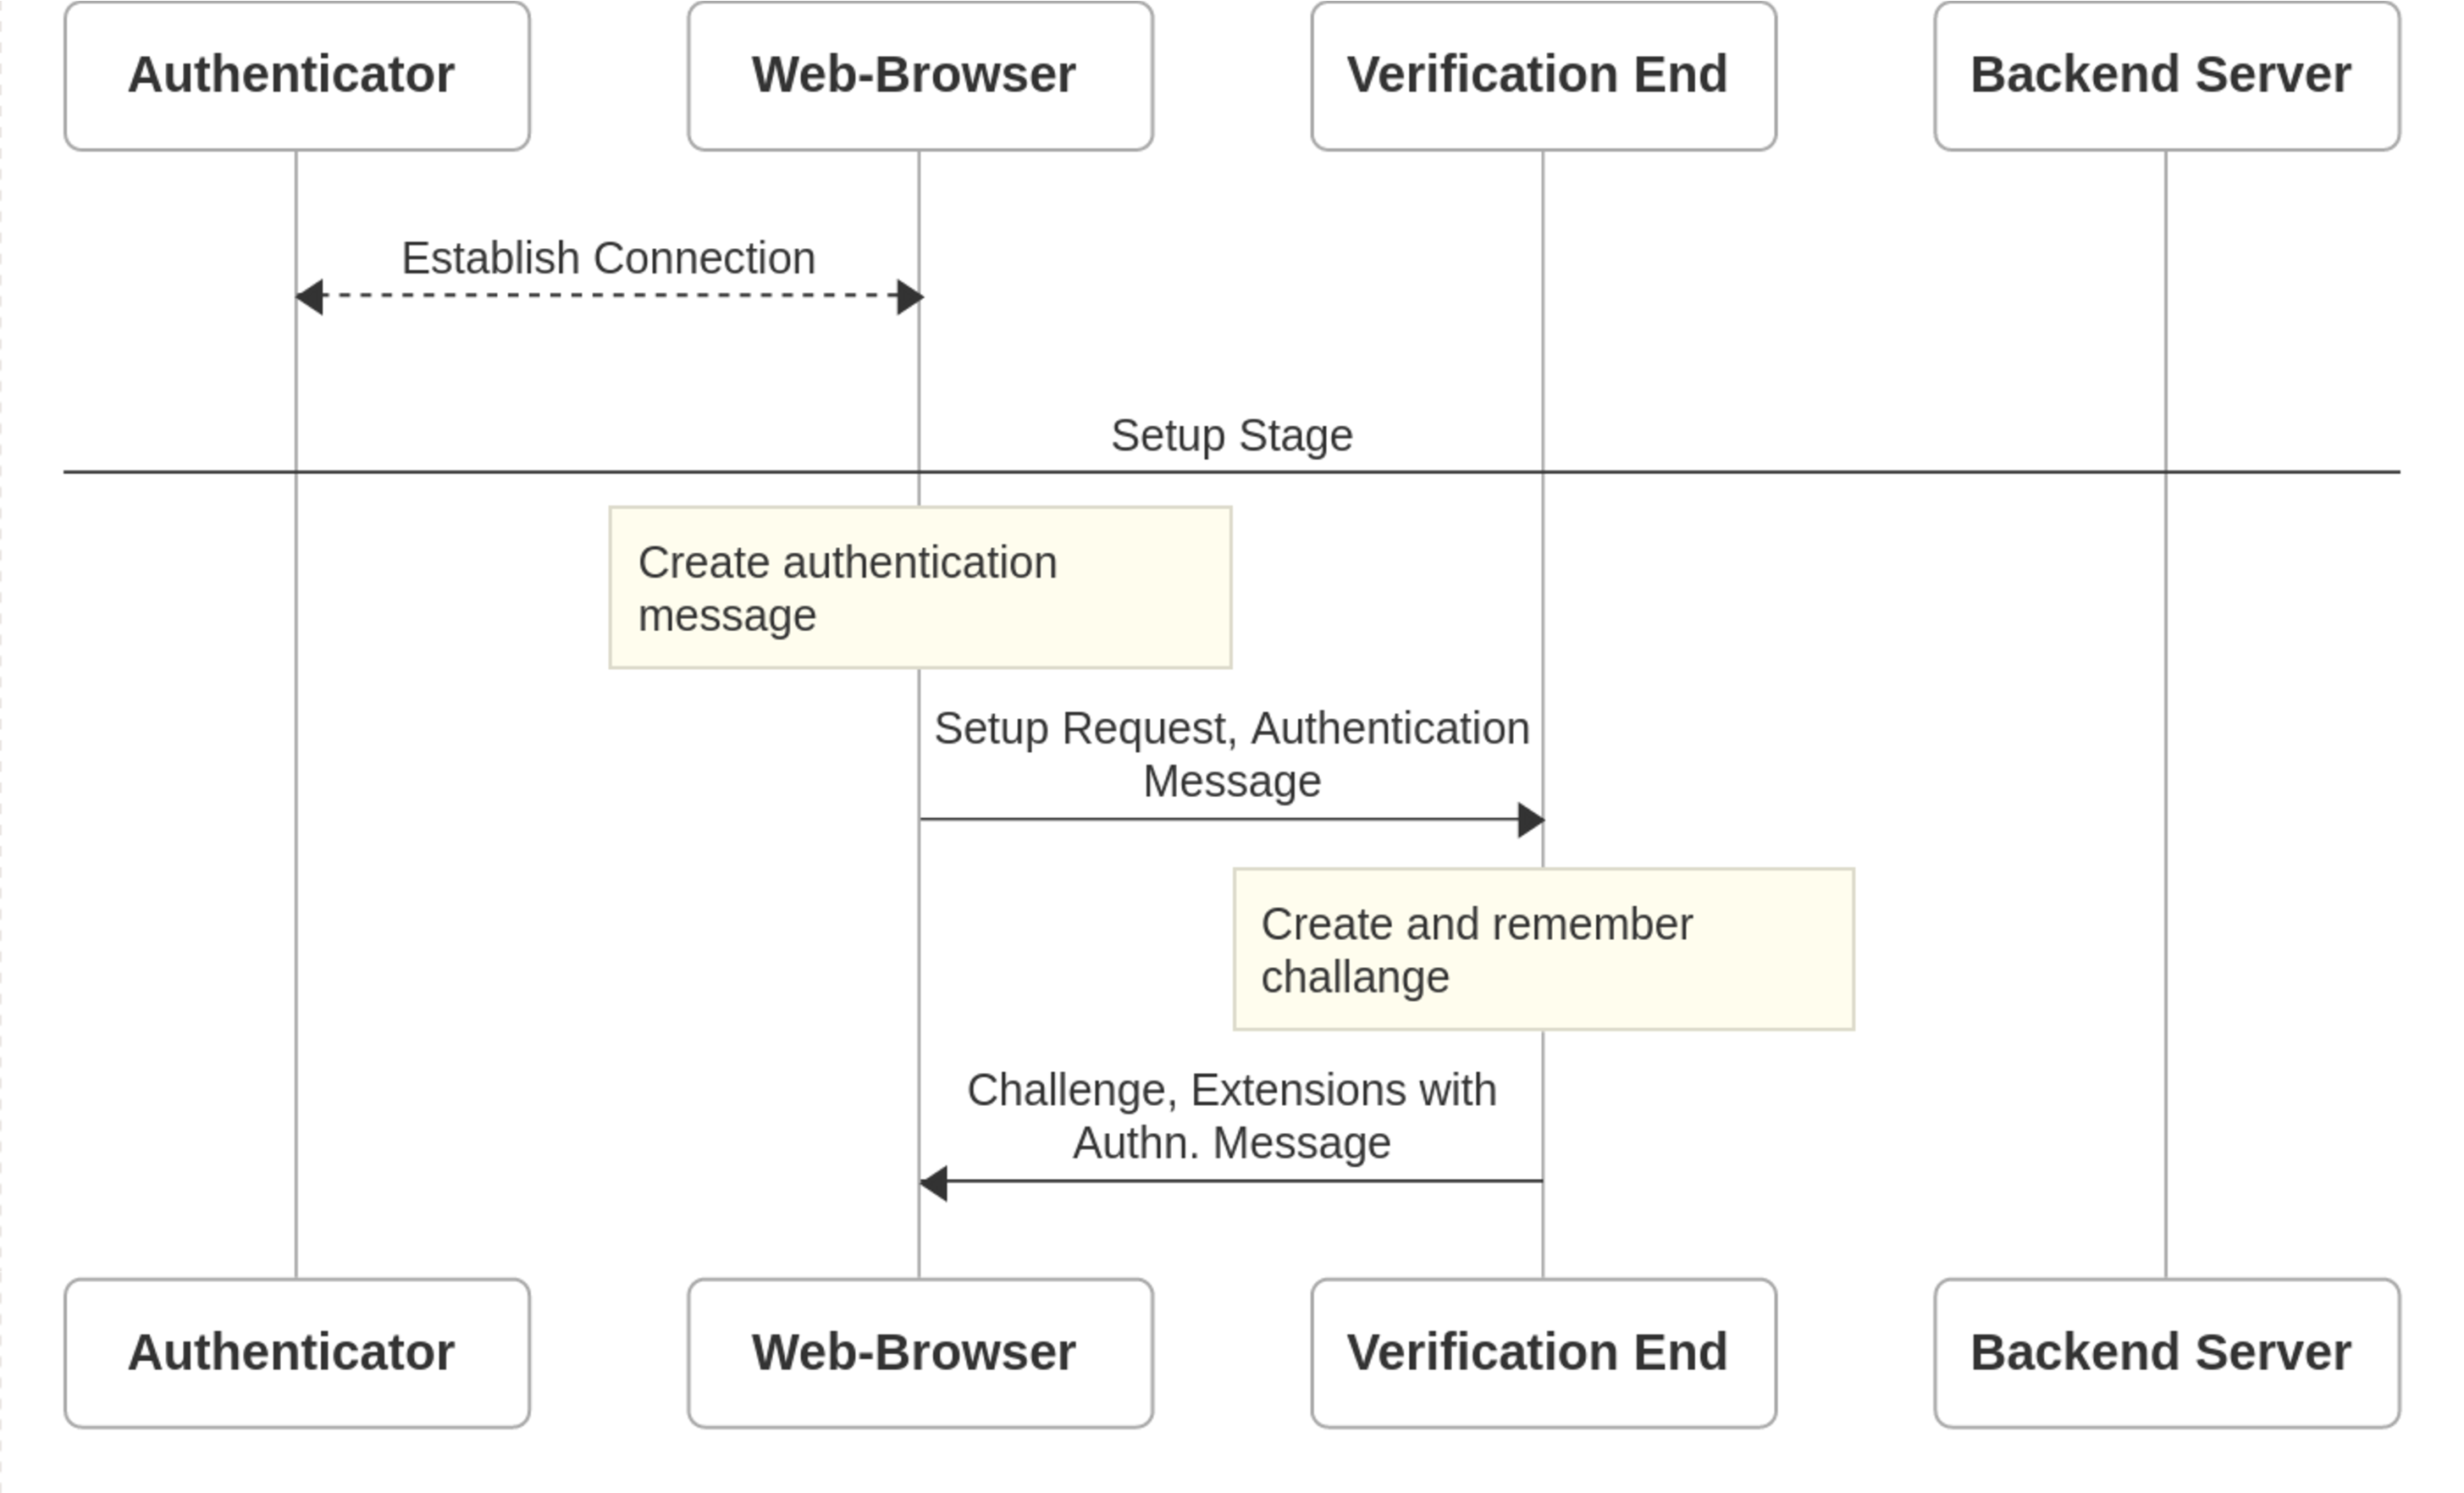
\includegraphics[width=16cm]{txauthn_flow_setup_swimlanes}
  \caption{The flow of events during the setup stage of WebAuthn transaction authentication.}
  \label{Fig:TxAuthnFlowSetup}
\end{figure}


% TODO: Talk about server-side rendering preloading

The setup for a transaction authentication event originates from the frontend webpage on the web-browser. There are several ways to setup a WebAuthn transaction event, but the contents being exchanged are all the same. More commonly, setup occurs lazily where the frontend waits for the user to initiate an operation protected by transaction authentication before initiating the setup. Or it may occur eagerly where the frontend preemptively initiates the setup, without knowing whether the user will even perform any secured operation on the webpage. 

Figure~\ref{Fig:TxAuthnFlowSetup} illustrate the setup stage of a transaction authentication event. The setup begins with a POST request sent to \sys{}. The payload for the setup POST request is an authentication message that will eventually be displayed to the user on their hardware device. The message is constructed from user input and additional information contained in the HTML of the webpage, but in all three case studies of this thesis, that was always enough. In response to the POST request, the frontend receives a few parameters:

%% 
%% \iffalse
%% \begin{lstlisting}
%% type PublicKeyCredentialRequestOptions struct {
%% 	Challenge          Challenge                   
%% 	Timeout            int                         
%% 	RelyingPartyID     string                      
%% 	AllowedCredentials []CredentialDescriptor      
%% 	UserVerification   UserVerificationRequirement 
%% 	Extensions         AuthenticationExtensions    
%% }
%% \end{lstlisting}
%% \fi
%% 

\begin{enumerate}[nosep]
\item A random \lstinline{challenge} nonce: The firewall remembers it locally in the session data associated with the request. When the firewall processes the protected request, it will verify that the challenge included in the returned authentication data matches the one previously sent and remembered in the session. An adversary cannot intercept and replay old protected requests since it is exceedingly unlikely that future challenges from the firewall will exactly match the challenge in the intercepted request.

\item An \lstinline{extensions} field: The firewall transforms the authentication message sent to it into a WebAuthn-compatible form for the hardware authenticator. It then places it into the \lstinline{extensions} field, which the authenticator reads and handles as a transaction authentication event.

\end{enumerate}

%% 
%% \iffalse
%% This field contains the authentication message. The firewall transforms this message into a webauthn-compatible form for the hardware authenticator device., so that the device
%% \fi
%% 

%% 
%% \iffalse
%% There are other fields returned as a part of the setup, but they are mostly for plumbing. They delineate how the hardware device should respond when authenticating the webauthn transaction.
%% \fi
%% 

%% 
%% \iffalse
%% The other fields are mostly for plumbing. The \lstinline{Timeout} requires an authentication response with that amount of time. The \lstinline{RelyingPartyID} identifies the backend. The \lstinline{AllowedCredentials} identifies with which cryptographic key the user can sign the response. The \lstinline{UserVerification} tells the hardware authenticator that the user must physically confirm ``yes'' or deny ``no'' a request and is usually set to \lstinline{true}. The \lstinline{Extensions} includes a signal that transaction authentication is to be performed with the authentication message sent to the firewall.
%% \fi
%% 

\section{Cryptographic Attestation}\label{Sec:CryptographicAttestation}

\begin{figure}
  \centering
  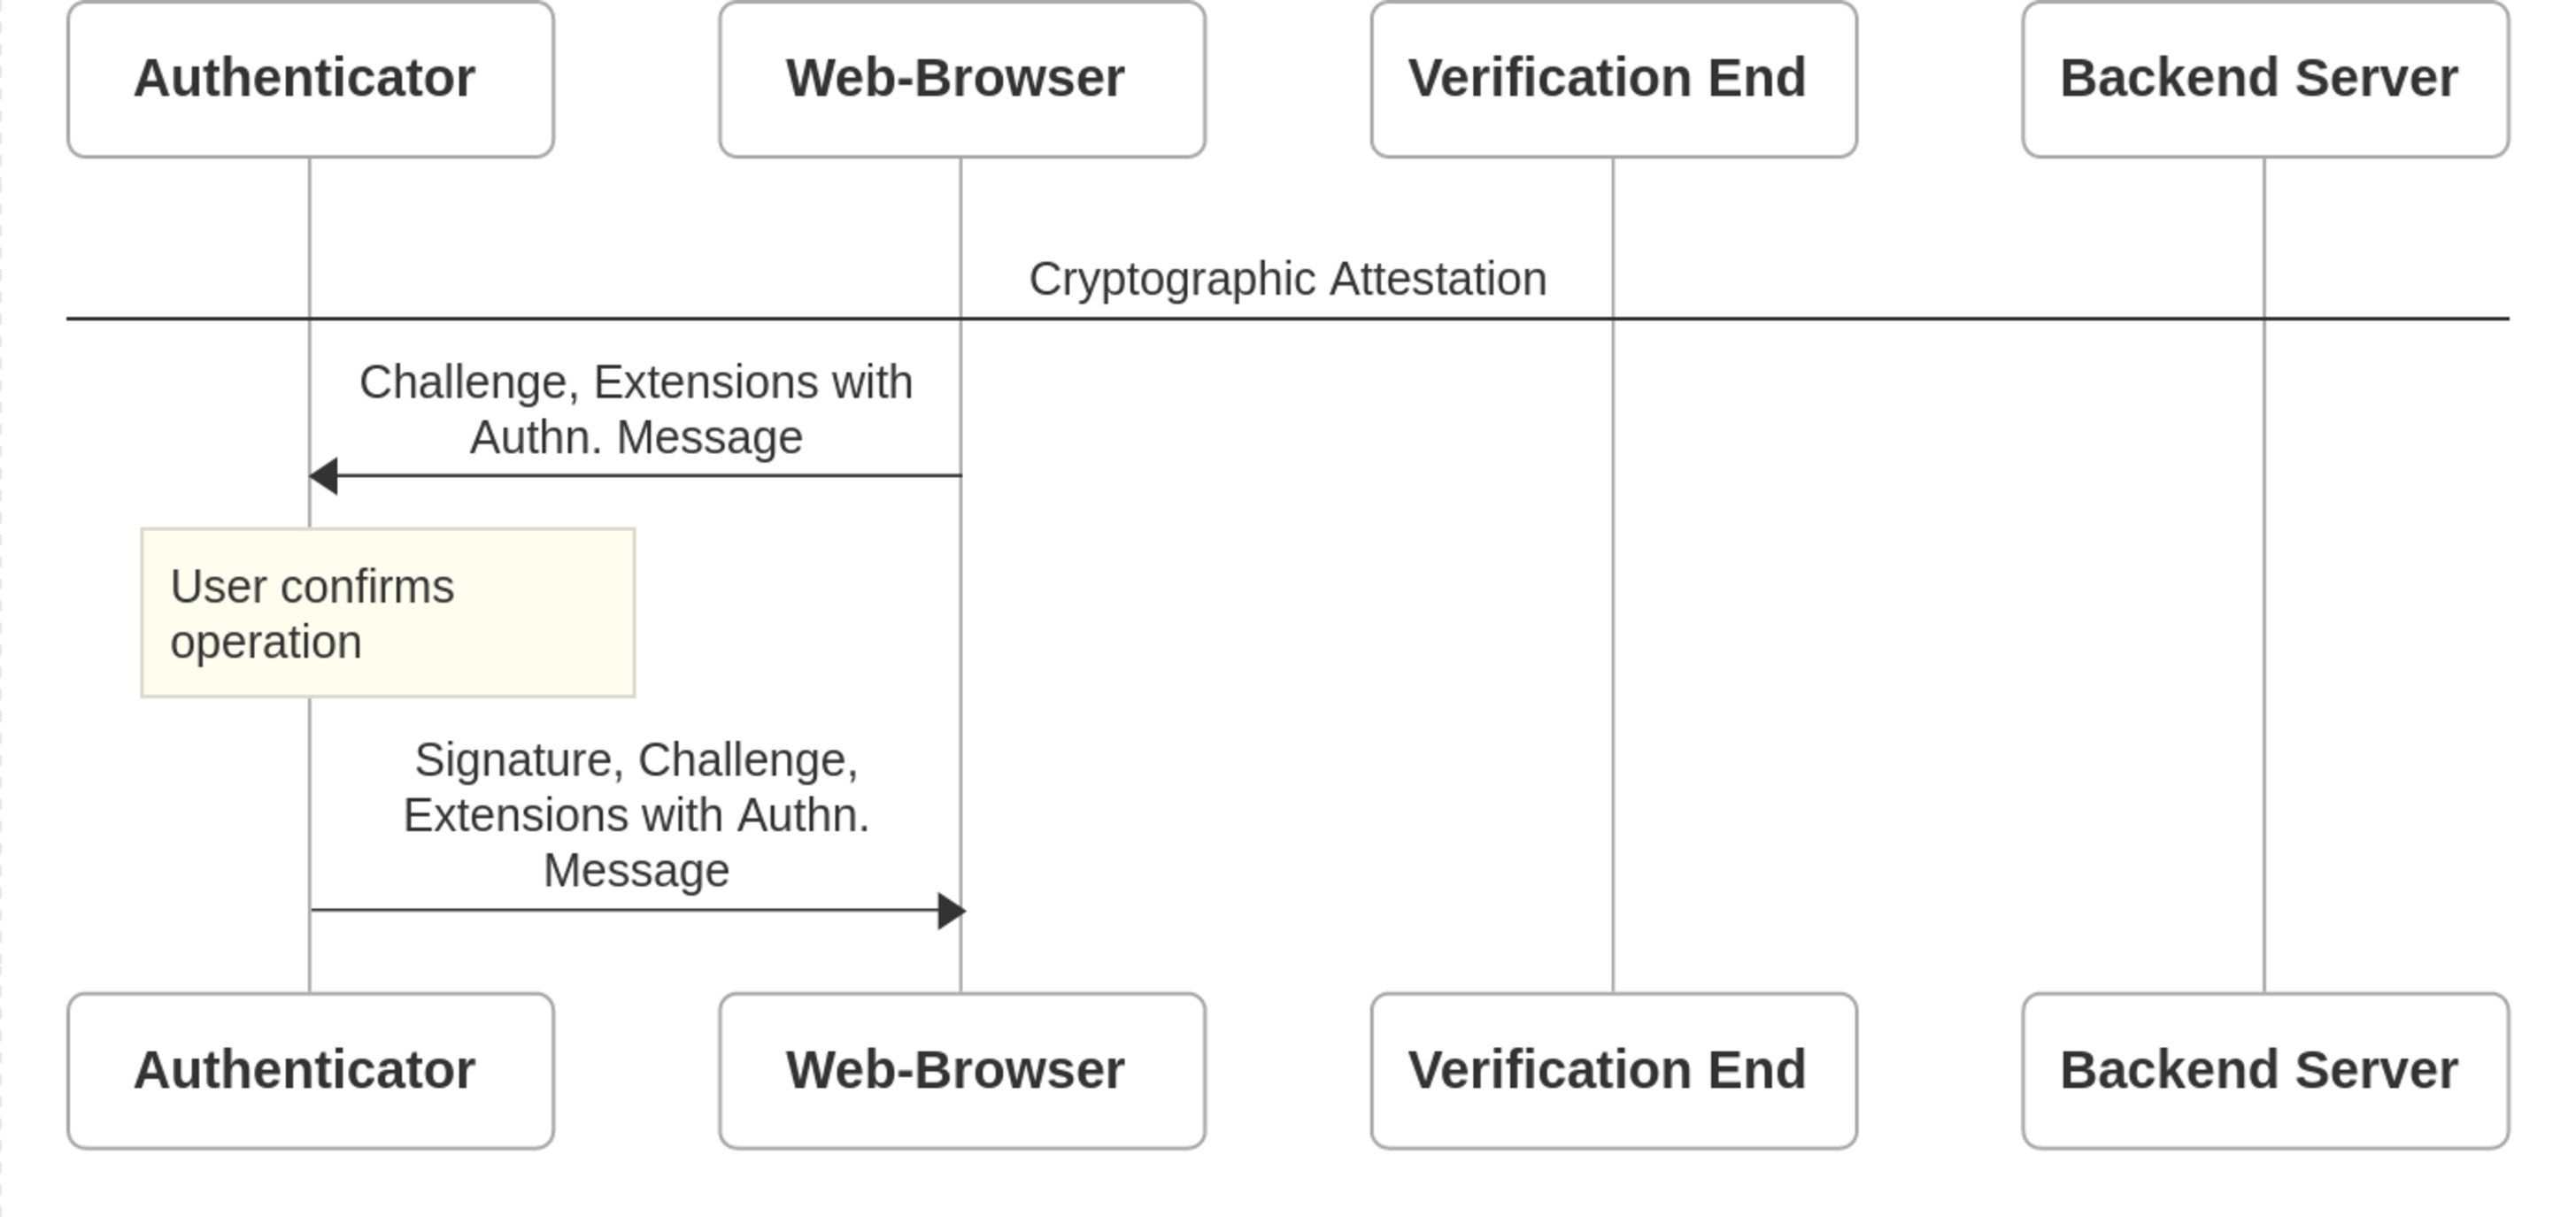
\includegraphics[width=16cm]{txauthn_flow_cryptoattest_swimlanes}
  \caption{The flow of events during the cryptographic attestation stage of WebAuthn transaction authentication.}
  \label{Fig:TxAuthnFlowCryptoAttest}
\end{figure}

The request options from \sys{} go through the frontend and are passed on to the hardware authenticator device. The threat model assumes that only the firewall, backend and hardware authenticator are secure. At any point, the frontend or web-browser could modify these options, but any tampering will be detected later on and denied authorization. 

Figure~\ref{Fig:TxAuthnFlowCryptoAttest} outlines the role of the hardware authenticator. The hardware device parses the request options, extracts from the \lstinline{extensions} field the authentication message and presents that to the user. The authentication message is in the form of a confirmation for some requested operation and is answered either by ``yes'' or ``no''. If the user attests ``yes'', the hardware device cryptographically signs a data object, which is returned as an additional field within the HTTP request to \sys{} for verification.

The response of the hardware authenticator includes a \lstinline{clientDataJSON} object containing the authentication message displayed to the user a well as the \lstinline{Challenge} from the setup stage. A cryptographic signature of the \lstinline{clientDataJSON} is also included. The signature is computed using Elliptic Curve Digital Signature Algorithm (ECDSA) paired with the SHA-256 hash function. There are other fields, as well, for plumbing to help \sys{} know what parameters to use to validate this response.

%% 
%% \iffalse
%% % TODO: Make this typescript highlighting
%% \begin{lstlisting}
%% const credential: PublicKeyCredential = {
%%     id: string, // base64 encoded
%%     rawId: []bytes,
%%     response: {
%%         attestationObject: []bytes,
%%         clientDataJSON: {
%%             challenge: string, // base64 encoded
%%             clientExtensions: []bytes,
%%             hashAlgorithm: string,
%%             origin: string,
%%         },
%%     },
%%     type: 'public-key',
%% };
%% \end{lstlisting}

%% The \lstinline{clientDataJSON} contains the \lstinline{clientExtensions} which is the data displayed to the user as well as the \lstinline{challenge} from the setup stage. The cryptographic signature of the \lstinline{clientDataJSON} is included in the \lstinline{attestationObject} and uses the Elliptic Curve Digital Signature Algorithm (ECDSA) paired with the SHA-256 hash function. The other fields are for plumbing and help the firewall know what parameters to use to validate this authentication data object.
%% \fi
%% 

\section{WebAuthn Firewall Verification}\label{Sec:WebauthnFirewallVerification}

\begin{figure}[h]
  \centering
  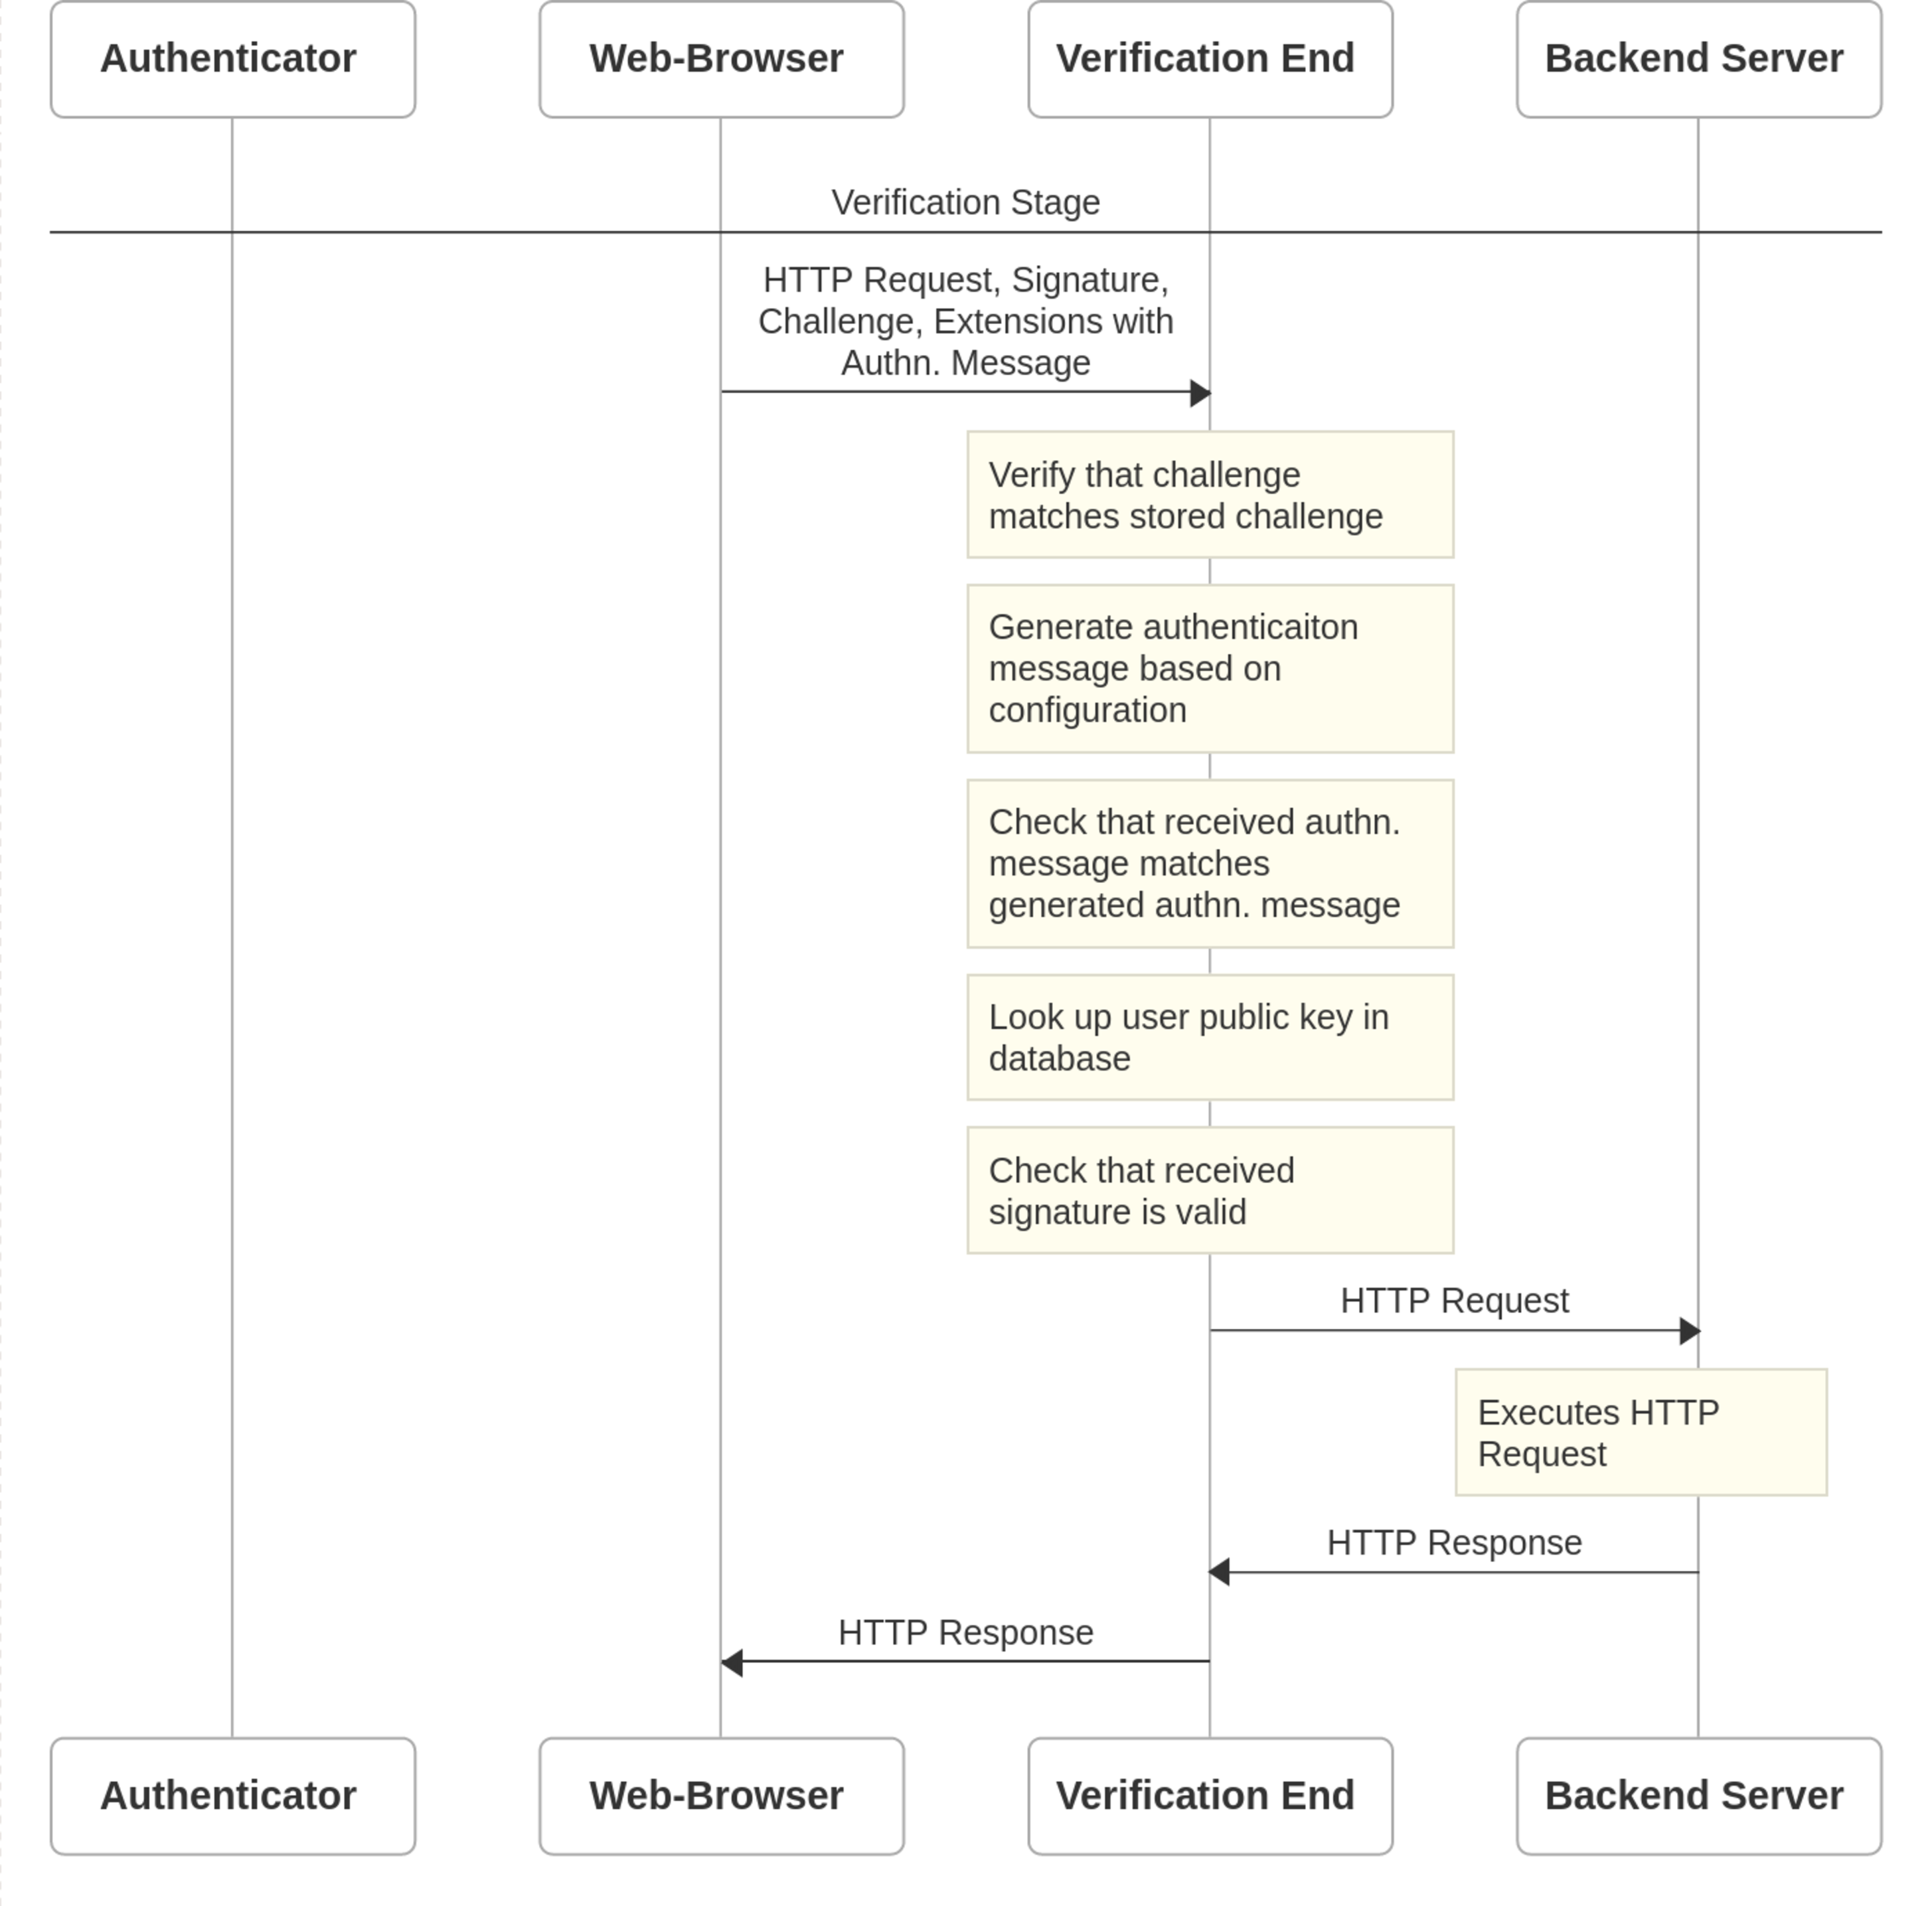
\includegraphics[width=16cm]{txauthn_flow_verification_swimlanes}
  \caption{The flow of events during the verification stage of WebAuthn transaction authentication.}
  \label{Fig:TxAuthnFlowVerification}
\end{figure}

\sys{} receives an HTTP request on a protected route with all of its usual parameters plus the authentication data object. The firewall must verify the integrity of this object as well that it corresponds with the intent of the HTTP request. In other words, it must detect whether any code not in the trusted computing base, such as the frontend, tampered with the authentication data. 

%% 
%% \iffalse
%% Also, it must make sure that the operation the user attested to on their hardware device that resulted in this authentication data object is in fact the operation to be performed if the protected HTTP request were to be permitted through. 
%% \fi
%% 

Figure~\ref{Fig:TxAuthnFlowVerification} illustrates the main steps of the verification stage. The three main steps are verifying the challenge, the authentication message and the authentication data signature:

\begin{enumerate}[nosep]

\item Checking the challenge is a simple comparison between the challenge received \lstinline{challenge} and the \lstinline{storedChallenge} in the firewall's session data. This protects against replay attacks.

%% 
%% \iffalse
%% \begin{lstlisting}
%% // Verify the challenge
%% Challenge := c.ClientDataJSON.Challenge
%% if strings.Compare(storedChallenge, Challenge) != 0 {
%% 	err := ErrVerification.WithDetails("Error validating challenge")
%% 	return err
%% }
%% \end{lstlisting}
%% \fi
%% 

\item Checking the authentication message is more involved. The firewall is configured per route how to generate an expected authentication message based on the HTTP request parameters. This generated authentication message must unambiguously encapsulate the entire intent of the request. Details are further discussed in Section~\ref{Sec:AuthenticationMessage}. Then it is a simple comparison between the received \lstinline{clientMessage} and the \lstinline{generatedMessage}. This makes sure the user authenticated a message that faithfully represents the intent of the HTTP request.

%% 
%% \iffalse
%% \begin{lstlisting}
%% // Verify the authentication message
%% clientMessage := c.ClientDataJSON.Extensions["txAuthnSimple"]
%% if strings.Compare(generatedMessage, clientMessage) != 0 {
%% 	err := ErrVerification.WithDetails(
%%               "Error validating authentication message")
%% 	return err
%% }
%% \end{lstlisting}
%% \fi
%% 

\item Checking the authenticating data signature involves invoking cryptography library utilities. This validates the integrity of the entire authentication object to prove that it was not tampered with. The \lstinline{clientDataJSON} was signed by the hardware authenticator. The firewall has the public key of the hardware authenticator, so it can see if the \lstinline{clientDataJSON} indeed corresponds to the signature attributed to it.

\end{enumerate}

%% 
%% \iffalse
%% \begin{lstlisting}
%% // Verify the signature

%% // The data signed by the hardware authenticator
%% clientDataHash := sha256.Sum256(c.ClientDataJSON)
%% sigData := append(p.Raw.AssertionResponse.AuthenticatorData, 
%%                   clientDataHash[:]...)

%% // The user's public key stored in the firewall
%% key, err := webauthncose.ParsePublicKey(credentialBytes)
%% valid, err := webauthncose.VerifySignature(
%%                  key, sigData, p.Response.Signature)
%% if !valid {
%% 	return err
%% }
%% \end{lstlisting}

%% Setup can occur eagerly where the web-browser immediately performs the setup without the user initiating any operation protected by transaction authentication.

%% If not, it will deny the request from continuing through.

%% The frontend only has access to the information it displays in the HTML to the user, 

%% The data displayed to the user along with its respective signature is included in the \lstinline{response} field. The hardware device signs
%% \fi
%% 
